\documentclass[conference]{IEEEtran}
\IEEEoverridecommandlockouts

\usepackage{cite}
\usepackage{amsmath,amssymb,amsfonts}
\usepackage{algorithmic}
\usepackage{graphicx}
\usepackage{textcomp}
\usepackage{xcolor}
\usepackage{array}

\newcolumntype{P}[1]{>{\centering\arraybackslash}p{#1}}

\def\BibTeX{{\rm B\kern-.05em{\sc i\kern-.025em b}\kern-.08em
    T\kern-.1667em\lower.7ex\hbox{E}\kern-.125emX}}
\begin{document}

\title{Clustering Source Code Comments}

\author{\IEEEauthorblockN{Welisarage Sudara Fernando}
\IEEEauthorblockA{\textit{Dept. of Electrical and Computer Engineering} \\
\textit{University of Auckland}\\
Auckland, NZ 1010 \\
wfer594@aucklanduni.ac.nz}
}

\maketitle

\begin{abstract}
Text clustering and classification techniques are used in characterising text documents into one or more categories based on various factors. This study focuses on classifying source code comments into a set of categories by utilising several natural language processing techniques such as TF-IDF vectorising, stop words elimination and frequency distribution count of token in the text document. Furthermore, the comments to perform classification are also collected by implementing a source code scanner for Java.
\end{abstract}

\begin{IEEEkeywords}
text classification, comments, tf-idf vectorising, dbscan, k-means
\end{IEEEkeywords}

\section{Introduction}
%what are we doing

Data classification highlights the relationships between data points. It uncovers information otherwise hidden in plain-sight which can be visualised and processed to make better-informed decisions. Text clustering is a form of data classification which divides a set of text documents into one or more categories based on their underlying linguistic content. It can be visualised as a mapping function which maps the given documents into categories. It can be one-to-one as well as one-to-many \cite{5557448}. The semantic factors that influence text classification results are discussed, focusing on the ones that apply on "short text"s, such as source code comments which are usually in the range of 100 to 150 words.

Natural Language Processing (NLP) has been a vital topic in computer science. It involves analysing human languages and recognising the connotative idea of text documents. NLP is a subfield of Artifical Intelligence (AI) and Machine Learning (ML) which extends a computer program's understanding of human languages. It powers several linguistic tasks such as text summarization, classification, translation and manipulation. Human languages are inherently complex. Some complexities of the English language are different literal meaning from the actual implied meaning (idioms and slang), different meaning of the same word depending on the context and different style of writing (American and British). However, advanced NLP techniques have progressively enabled the understanding of the intricate languages \cite{4368002} which innately enables excellent text manipulation using computer systems. This paper explores different NLP techniques and algorithms which can be utilized for meaningful text classification. 

The clustering algorithms discussed in this research are based on \textit{unsupervised learning} methods which utilises a set of features F\textsubscript{1},F\textsubscript{2},F\textsubscript{3}...F\textsubscript{n} obtained from \textit{n} observations to produce a meaningful visualization of data. This is opposed to \textit{supervised learning} which predicts a response \textit{R} over the feature set F\textsubscript{1},F\textsubscript{2},F\textsubscript{3}...F\textsubscript{n} using a set of \textit{f} features \{F\textsubscript{1},F\textsubscript{2},F\textsubscript{3}...F\textsubscript{n}\} measured from \textit{n} observations and a response relation \textit{R\textsubscript{R}} which is also measured on the same \textit{n} observations \cite{book_1}.

The only input for an \textit{unsupervised learning} approach is the dataset. The dataset for this project is obtained through a source code scanning program designed to scan through Java source code. An \textit{unsupervised learning} procedure does not require a pre-determined response relation (a model) since the process does not involve in any prediction. In a \textit{supervised learning} environment, the results can be cross-validated with the predetermined model. However, in an \textit{unsupervised} approach, there is no universally accepted mechanism to validate the results since the problem itself was unsupervised without an initial model \cite{book_1}. The algorithms used in this research visualise the results, but unable to cross-validate due to the unsupervised nature of the problem. 

Two main outcomes of this project are retrieving comments from source code files and classifying them into several categories. 

\subsection{Retrieving source code comments}

The dataset was obtained through a source code scanner program which was designed to scan through a given set of Java source code files collecting both single-line as well as multi-line comments. More than 5,000 Java source files were obtained from several well-established and maintained open source projects such as Firebase Admin API (Java), Android Open Source Project and Apache Hadoop. The comments scrapped from the used files were written in English which adheres to correct English language grammar and semantics.  

\subsection{Comment clustering}

The collected comment data is then processed using various NLP techniques and data cleansing methods. After cleansing it is represented it as \textit{n x n} matrix. The matrix is then vectorised using a TF-IDF Vectoriser and then fed into the algorithm. The DBSCAN clustering algorithm was used as the clustering algorithm for this project. Finally, the result set is then examined to identify and visualise the cluster output. 

\section{Literature Review}

\subsection{Retrieving source code comments}

Source code parsing and lexical analysis of the programming languages are used in many software products such as Integrated Development Environments (IDE) and other text editors to provide visual feedback of the code that a developer is working on. These tools utilise regular expressions and other language-specific tools to construct a data structure called \textit{abstract syntax tree} (AST) which is composed of a sequence of characters \cite{BADROS2000159}. Several authors have attempted to design software tools to obtain an AST from Java source code.

One such implementation is to obtain an XML view of the Java source code, named JavaML \cite{BADROS2000159}. The authors formalise a \textit{document type definition} (DTD) which describes the conversion of Java grammar into XML nodes. Then a computer program based on IBM Jikes Java compiler framework \cite{ibm-jikes} was used to parse the standard Java source files and convert them into JavaML documents. These JavaML documents can be utilised by other programs which support XML file parsing. Java is a live language which gets continuously updated. Hence it is vital to keep the language parsers up to date which is also being discussed by the authors in their paper. However, the proposed algorithm only supports Java 5.0 and is unable to process the new Java lexical structure introduced in newer Java versions. Also, the suggested procedure generates a complex and bulky XML document even for simpler Java source code. XML itself is verbose and converting Java source with all its individual properties result in a massive XML document which makes it challenging to cross-validate. 

Contrary to AST, Token-based source code feature identification is also found in the literature. The token-based approach is linear complexity in both time and space and does not require the whole document to be parsed at once \cite{4023995}. It even works when the source code is syntactically incorrect or incomplete. It is more suitable to identify a particular language feature (such as individual methods, variables or comments). AST-based procedures usually traverse the whole document several times to classify the distinct language components whereas the token-based approaches tokenise the source code to recognise the required language feature. 

An open-source library named \textit{"javalang"} provides a lexer and a parser for Java 8.0 syntax. \textit{"javalang"} uses token-based feature extraction to scan and tokenise a Java source code and represents it in a tree data structure \cite{java-lang}. It also provides a Python API to access the properties and methods listed in the Java source code. However, one shortcoming of this library was that it was unable to recognise multi-line comments. 
 
\subsection{Comment clustering}

Several text clustering algorithms such as K-Means, DB-SCAN and FTSC exist in the current literature. These algorithms are mainly categorised into prototype-based, density-based and hierarchical clustering. Prototype-based algorithms such as K-Means assigns each document into its nearest initial prototype cluster. Density-based clustering algorithms such as DBSCAN, separate documents into subsets of similar densities \cite{5659055}. These algorithms differ from each other based on several factors such as scalability, use case and geometry. Each algorithm also requires a different set of parameters as inputs. 

The frequent terms in text clustering is a common factor analysed by several algorithms. Frequent term Set-based clustering (FTSC) was introduced by X Liu et al. which uses frequent term sets for text clustering \cite{1527337}. FTSC uses a part-of-speech tagging system to segment the terms of a text document and use a discrimination value (DV) of feature terms to find words which can reflect the caption of a text. The DV value represents a word token's ability to distinguish unique document with different contents when it is used to identify the content. Furthermore, Frequent Term Set-based Hierarchical Clustering algorithm (FTSHC) modelled after FTSC can produce overlapping clustering results which increase its reliability and accuracy. Authors claim that it is both faster and reliable than the K-Means algorithm. 

FTSC improves the efficiency of clustering by choosing a set of frequent terms based on its appearance frequency as the candidate set without immediate clustering of the documents with high dimensions. Mining of the frequent terms is a two-step process where all the frequent items found in the text are filtered according to a predetermined threshold (internally known as \textit{min\_sup}) \cite{1527337}. Then the general association rules are obtained for each filtered item set adhering to the rules defined in the Apriori algorithm. Each frequent term in frequent term set \textit{\{F\}} forms a clustering category where each category \textit{\{f\textsubscript{i}\}} has the least mutual overlap \cite{1527337}. It shows that there is no much difference in the clustering results obtained from FTSC and K-Means algorithms according to the quantitative analysis conducted by the authors using F-Measure on two datasets (namely \textit{NTCIR-3} and \textit{Reuters-21578}). However, due to the nature of the frequent term selection algorithm used in mining the datasets, FTSC is more optimised for text documents with longer and larger text data \cite{1527337}.

Density-based spatial clustering of applications with noise (DBSCAN) is a data clustering algorithm which is heavily adopted for text clustering. It requires two main parameters; a point neighbourhood and the minimum number of points (\textit{min\_sample}) in the neighbourhood. The cohesion of the result depends on this minimum point value \cite{5659055}. The algorithm starts at an arbitrary position and if \textit{min\_sample} $\leq$ number of points in the initial position, then a cluster is formed. Otherwise, the point will be marked as noise and will select another point to repeat the process. DBSCAN produces clusters of arbitrary shape and is more sensitive for datasets with noise. 

The selection of the \textit{min\_sample} and the minimum neighbourhood value (\textit{eps}) depends on the dataset used. Setting the \textit{min\_sample} to 1 does not make any sense since every document in the corpus will then be considered as a cluster by itself. It is usually recommended to set this value to a minimum 3. But it may be possible to set a generous amount for a bigger dataset or datasets with more noise and duplicates.  The eps value affects the number of clusters produced in the result (discussed in \textsc{Section V}). If the chosen amount is too small, a large part of the data will be discarded as noise. If it is too big, then the clusters will merge affecting the accuracy of the outcome.

\section{Dataset preparation}

The primary goal of this research is to mine comment data from a given set of Java source files and to cluster them based on their linguistic content. A Java source code scanning program was developed in Python to scan through source files and collect both single-line as well as multi-line comments. The program uses a token-based source code scanning approach since it only targets a specific language component (i.e comments). AST traverses the source file several times to identify all the language components which is an overkill for this research. Token-based approach also dramatically reduces the time and memory requirements of the scanning program \cite{4023995} which is essential because the program has to scan an adequate amount of source files to obtain comment data for a meaningful clustered result set.

\subsection{Comment data collection}

The program scans the source files and identifies the comment start and end tokens depending on the comment type. It then starts capturing the comment as soon as it detects the start character and ends the comment when it meets the end character. The start character may appear in any arbitrary location in the scanned line. In case of the multiline comments, the star (*) character that appears in between the lines are omitted. To minimise unwanted omissions, it gets excluded only if it is followed by a line-end character. 

\begin{table}[!h]
\renewcommand{\arraystretch}{1.3}

\caption{Start and end tokens for Java comments}
\label{table_example}
\centering
\begin{tabular}{c|c|c}
\bfseries Comment Type & \bfseries Start Character & \bfseries End Character\\
\hline
Single-line & // & Line end charactor\\
\hline
Multi-line & /* & */
\end{tabular}
\end{table}

The collected comment data is then stored in a Python dictionary along with a reference to the file. 

\begin{figure}
\centerline{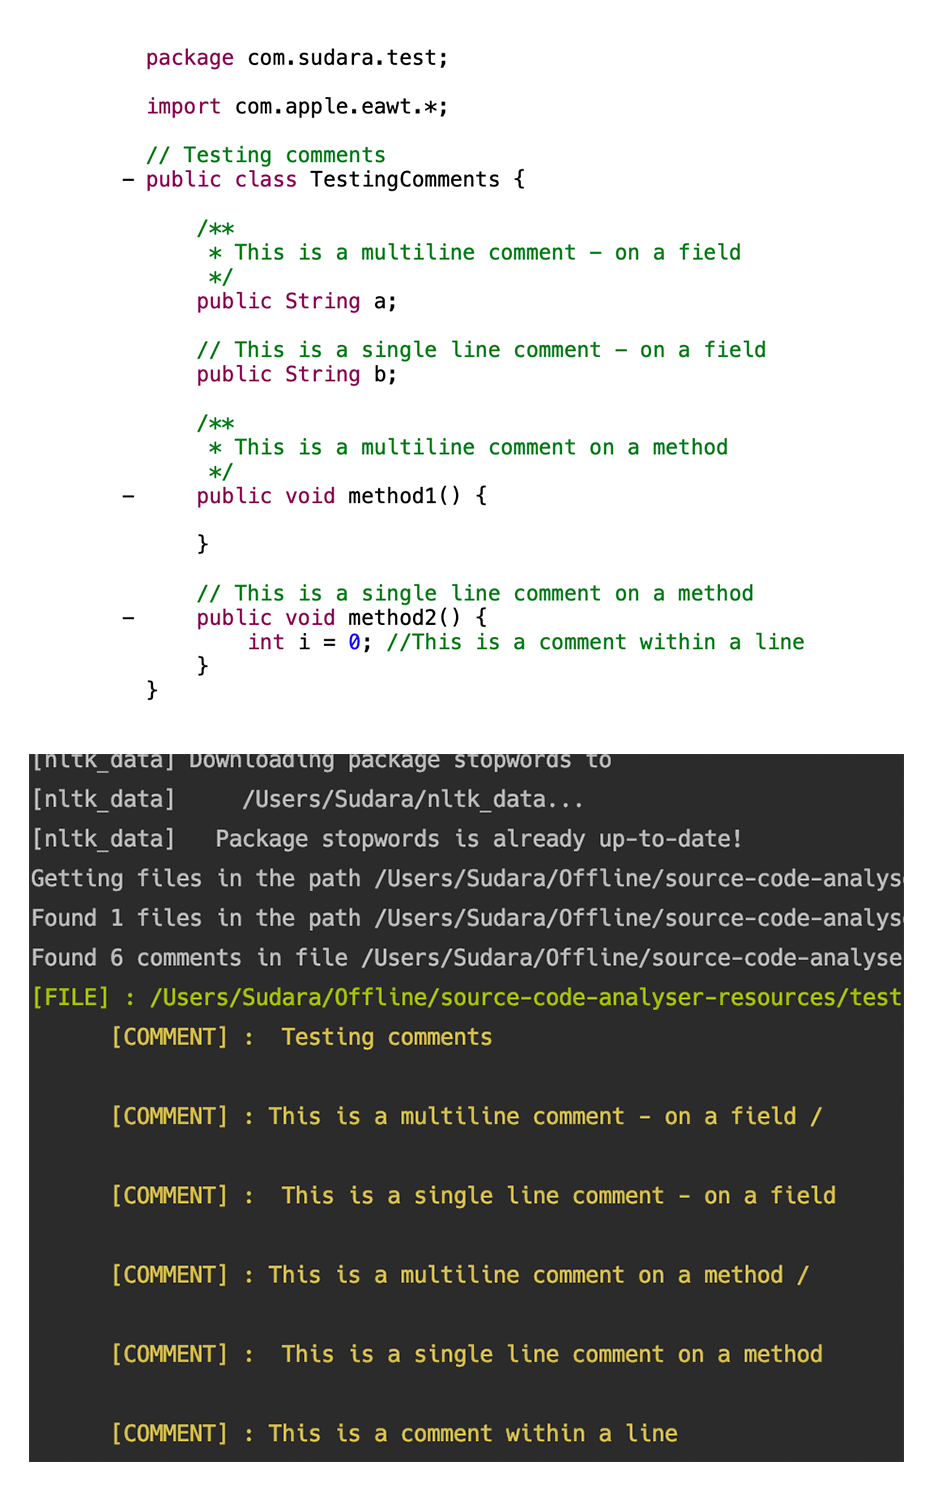
\includegraphics[width=6cm, height=9cm]{graphics/java-program_combined.png}}
\caption{Comment scanning example}
\label{fig}
\end{figure}

\subsection{Data cleaning}

Data cleaning is an essential step in text clustering process. Text clustering, specially density-based clustering algorithms cluster documents depending on the neighbourhood spacial size. Several common English language terms such as articles, pronouns, prepositions and conjunctions can skew the results as they commonly occur in text documents. Also in most cases, the less frequent words in a sentence convey the meaning rather than the most occurring articles and pronouns. 

\subsubsection{Filtering stop words}

Stop words with a high count frequency occur in a variety of languages and texts. These words can skew the frequency counting and density based classifications. They appear in several places of the sentence yet fail to convey the meaning without other content words accurately. Examples for stop words in the English language include "of", "is", "the" etc. There are two possible ways to filter the stop words. One is to use a precompiled stop words dictionary and to refine the text document excluding the words found in the dictionary. The other option is to use a word frequency threshold where words with higher frequencies are considered stop words \cite{5635068}. 

The NLTK Python package, which is used for the clustering process uses a precompiled stop words dictionary. Once the \textit{"stopwords"} package is downloaded, the words can be filtered by specifying the language. 

\subsubsection{Stemming and lemmatization}

Both stemming and lemmatisation are used in English language text processing. Reducing a word by analysing its prefix or suffix into its stem or root is known as stemming. Words with the same meaning with different prefixes and suffixes can affect count frequency. For example, words \textit{"running"}, \textit{"ran"} and \textit{"runs"} represent the root word \textit{"run"}. These words would be counted as different unless they were stemmed into its roots. The information retrieval of the English documents is improved by 6\% - 8\% after using a stemming process \cite{6272740}. 

\textit{EnglishStemmer} from \textit{nltk.stem.snowball} package was used in the project for stemming the words into its root representation. 

\section{Document feature extraction}

After obtaining the dataset, the next step is to extract several document features. In this step, the raw text data will be transformed into feature vectors to be analysed by the clustering algorithm. 

\subsection{Bag of words representation}

The raw corpus data cannot be fed directly into most of the algorithms for analysis. It will have to be converted into fixed size numerical feature vectors for it to be processed and analysed. This conversion of raw text data into a collection of numerical feature vectors is known as "Bag of Words" ("Bag of n-grams") representation. The project applies a three-step conversion function. Firstly the words are tokenised into several token terms. Each of the tokens is given an integer id for later identification. Secondly, each token occurrence is counted and stored in a matrix (3D array). Finally, the counted tokens are weighted using TF-IDF as described below. The final matrix represents the input corpus as a set of numerical vectors. This matrix representation is then used by the DBSCAN algorithm to analyse and form the clusters. \cite{scikit-learn}

\subsection{Count vectors}

The count vector represents the frequency of a token occurrence in the given document. It is internally depicted as a matrix notation. In the matrix, a column is represented by a word or a term in the corpus and a row is represented by an individual document in the corpus. By examining each cell, we can identify the frequency count of a given word in the given text document.

\begin{figure}[!h]
\centerline{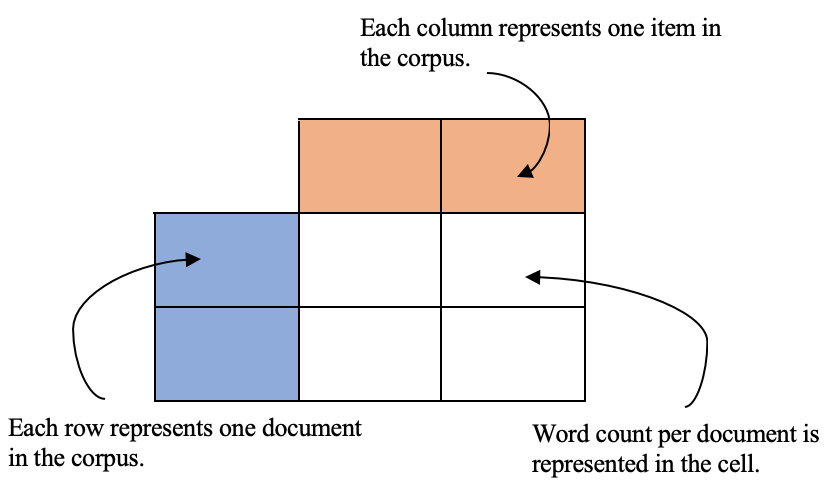
\includegraphics[width=5.75cm, height=3cm]{graphics/pic-1.png}}
\caption{Count vector representation in NLTK}
\label{fig}
\end{figure}
 
The \textit{CountVectorizer} class in the \textit{sklearn} package was used to obtain the count vector of the collected dataset.

\begin{figure}[!h]
\centerline{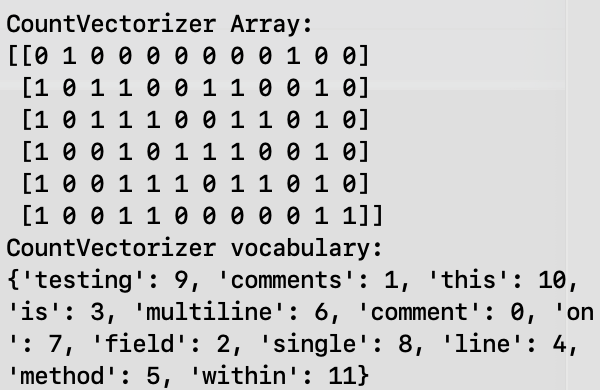
\includegraphics[width=5.75cm, height=3.75cm]{graphics/count-vec.png}}
\caption{Count vector representation in NLTK}
\label{fig}
\end{figure}

\subsection{TF-IDF vectors}

The TF-IDF (term-frequency times inverse document-frequency) represents the weight of a term in the entire document. TF-IDF weighting is essential because some scarce words in the language provide more meaning in the sentence than the other commonly occurring words. This aspect is ignored if we only count the occurrence frequency of a term rather than estimating the weighted value for contributing words.  

TF-IDF is a two-step calculation where the TF and the IDF scores are first calculated which is then multiplied to get the final score. TF (which stands for term frequency) of a term \textit{t} is calculated by dividing the count vector of \textit{t} in the document (\textit{d\textsubscript{x}}) by the number of documents in the entire corpus (\textit{d}) with term \textit{t}. IDF (which stands for inverse document frequency) of a term \textit{t} is computed as the logarithm value of the total number of the documents in the corpus divided by the total number of documents in the entire corpus (\textit{d}) with term \textit{t}. \cite{scikit-learn}

\begin{figure}[!h]
\centerline{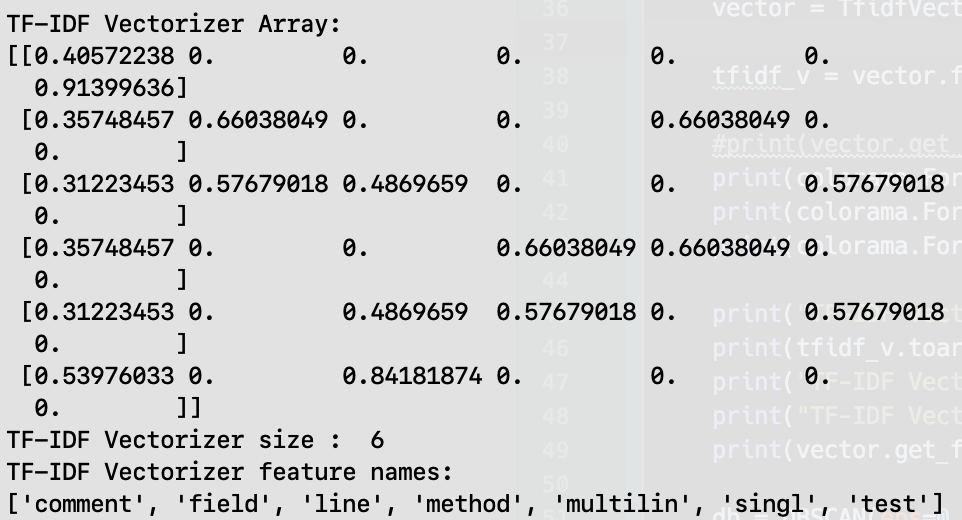
\includegraphics[width=7.75cm, height=4.25cm]{graphics/tfidf-vec.png}}
\caption{Count vector representation in NLTK}
\label{fig}
\end{figure}

\begin{equation}
\label{tf-calculation}
TF(t,d,d_x) = count(t,d_x) / count(t,d)
\end{equation}

\begin{equation}
\label{tf-calculation}
IDF(t,d) = log_e (count(d) / count(t,d))
\end{equation}

\begin{equation}
\label{tf-calculation}
TF-IDF(t,d) = TF(t,d,d_x) * IDF(t,d)
\end{equation}

The term \textit{t} in the TF-IDF score can be scoped into three levels; word level, n-gram level and character level. When the TF-IDF score is calculated considering the word level, it examines each word in all the documents. The n-gram level considers \textit{n} number of words determined by the user. Finally, at the character level, every character is recognised for the calculation. However, it seems that setting the scope depending on the size of the dataset yields better results. Character level should be considered with a small number of documents, while n-gram level should be considered with a more significant corpus. 

\begin{table}[!h]
\renewcommand{\arraystretch}{1.3}

\caption{TF-IDF scoping and cluster results}
\label{table_example}
\centering
\begin{tabular}{|P{1cm}|P{2cm}|P{2cm}|P{2cm}|}
\hline
 \bfseries TF-IDF scope level & \bfseries Corpus size & \bfseries Number of clusters & \bfseries Average documents per cluster\\
 \hline
 Word & 14,243 & 1,354 & 10.5\\
 \hline
 N-gram (2) & 14,243 & 654 & 21.71\\
 \hline 
 N-gram (3) & 14,243 & 432 & 32.81\\
 \hline
 N-gram (4) & 14,243 & 371 & 38.18\\
 \hline
 N-gram (5) & 14,243 & 332 & 42.64\\
 \hline
\end{tabular}
\end{table}

\section{Discussion}

The DBSCAN algorithm was used to cluster a sequence of comment documents. During the initial stage, the number of clusters is unknown. DBSCAN can cluster the documents by analysing the cluster density specified by the neighbourhood size. It creates an arbitrary number of clusters depending on the available data. Since the initial number of clusters is not available or restricted to a predetermined value, the algorithm can analyse the high-density areas to produce uneven and non-flat geometry cluster sizes. DBSCAN is also resistant to noise and robust to outliers. \cite{scikit-learn}

\subsection{Accumulated noise}

One crucial matter I noticed in the project was that the algorithm labels more data as noise if the dataset is small. This behaviour depends on the \textit{min\_samples} variable which determines the minimum documents required to form a cluster. The higher \textit{min\_samples} value, higher the number of documents classified as noise. If the \textit{min\_samples} value is 1, lots of clusters are generated with one document, which is expected since there aren't enough data in a small dataset. This phenomenon declines will the corpus size. Nearly 84\% of the documents in a corpus with around 3,000 documents were classified as noise. However, only 72\% were classified as noise in a corpus of size 14,000. 

\begin{table}[!h]
\renewcommand{\arraystretch}{1.3}

\caption{noise vs corpus size (\textit{min\_sample}=2)}
\label{table_example}
\centering
\begin{tabular}{|P{1.5cm}|P{1.5cm}|}
\hline
 \bfseries Corpus size & \bfseries Noise \% \\
 \hline
 1,231 & 95\% \\
 \hline
 2,156 & 89\% \\
 \hline 
 3,564 & 84\% \\
 \hline
 4,675 & 81\% \\
 \hline
 7,435 & 79\% \\
 \hline
 13,923 & 72\% \\
 \hline
 20,328 & 55\% \\
 \hline
\end{tabular}
\end{table}

\begin{figure}[!h]
\centerline{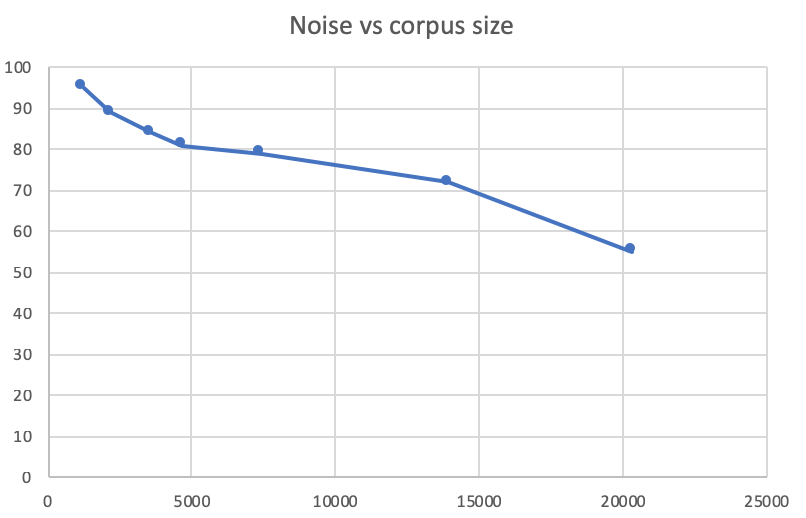
\includegraphics[width=6.75cm, height=4.25cm]{graphics/noise-vs-corpus-size.png}}
\caption{Noise vs corpus size}
\label{fig}
\end{figure}

Fig. 5 shows that the noise value decreases when a more significant corpus is used. This is expected because it should have access to a bigger dataset for the algorithm to form meaningful clusters. 
Most notably, the noise percentage started decreasing in an exponential rate when the corpus size is increased. In the range of size 1,000 to 4,000, it had a slow decline. However, it started plummeting when the corpus size was gradually increased up to 20,000. This must be because the algorithm has more data to form more clusters which otherwise would have labelled as noise. Since \textit{min\_samples} was set to 2, there wasn't enough data to create a valid cluster when the corpus size was below 5,000. 

\subsection{Cluster accuracy and cohesion}

The other parameter \textit{eps} value determines the similarity between two different samples. The accuracy of the classification mainly depends on this value. Less value indicates higher cohesion between the clusters and a higher value indicates a lower coherence. It is advised to determine this parameter depending on the dataset. By testing the algorithm with the obtained comment data (corpus of size nearly 14,000), it seemed that 0.7 is a better value for balancing the cluster cohesion and the validity.

\begin{table}[!h]
\renewcommand{\arraystretch}{1.3}

\caption{\textit{eps} value vs cluster formation}
\label{table_example}
\centering
\begin{tabular}{|P{1cm}|P{1.5cm}|P{1cm}|P{1cm}|}
\hline
 \bfseries eps value & \bfseries Corpus size & \bfseries Number of clusters & \bfseries Average documents per cluster\\
 \hline
 0.1 & 14,252 & 26 & 4.4\\
 \hline
 0.2 & 14,252 & 31 & 4.2\\
 \hline 
 0.3 & 14,252 & 41 & 4.0\\
 \hline
 0.4 & 14,252 & 83 & 4.16 \\
 \hline
 0.5 & 14,252 & 154 & 4.2 \\
 \hline
 0.6 & 14,252 & 258 & 4.3 \\
 \hline
 0.7 & 14,252 & 398 & 4.42 \\
 \hline
 0.8 & 14,252 & 561 & 4.78 \\
 \hline
 0.9 & 14,252 & 728 & 5.60 \\
 \hline
\end{tabular}
\end{table}

\begin{figure}[!h]
\centerline{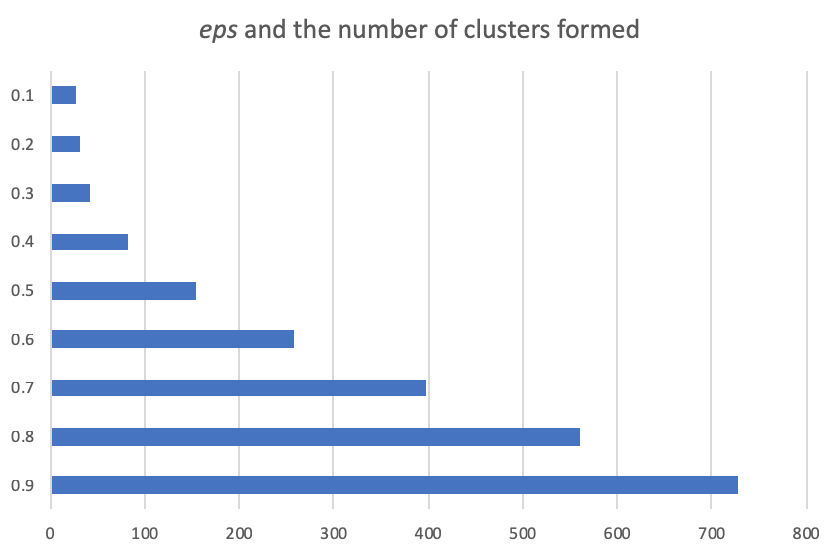
\includegraphics[width=6.75cm, height=4.25cm]{graphics/eps-num-of-clusters.png}}
\caption{Noise vs corpus size}
\label{fig5}
\end{figure}

The attached Appendix B lists examples of the clusters formed with the \textit{eps} value of 0.7 and \textit{min\_sample} of 3.

\section{Evaluation}

\subsection{Threats to validity}

As described in \textsc{Section V}, the clustering performance and accuracy is improved with a bigger corpus size. The more data the algorithm has access to, better the results are. However, text classification seemed a very resource intensive task which requires decent computing power. The algorithm was tested with a comment set of around 20,000 comments obtained from the Android Open Source Project, Firebase Admin API and Apache Hadoop Project. A typical computer with Dual-Core i5 processor and 8GB of RAM takes around 1 hour to process the given 20,000 comments. Using a variety of projects with a lot more comment data would produce a better-unbiased results set.

\subsection{Limitations}

One of the main limitations of the project is that it can only capture comments in Java source files. Additionally, the Java source file name should end with the \textit{.java} file extension. The program will omit all other files in the resources directory. This limitation dramatically restricts the application only to Java development teams. Even though not tested, some other Java-like languages such as Scala and Kotlin which also use the same commenting syntax should work with the program. However, this would still need a minor modification to allow the Scala and Kotlin files to be scanned by whitelisting the respective file extensions. 

Another limitation of this project is that the scanned corpus is limited to the amount of installed RAM in the running computer. Currently, all scanned data is processed while accessing it from the main memory. Even though this decision significantly reduces the execution time, it also limits the number of comments that the computer can handle. Due to this constraint, the program requires a significant amount of RAM to process extensive datasets. 

The program attempts to remove one to two-word comments which do not provide a context value. Also, licence text which usually appears at the beginning of the source file is also omitted. However, some developers tend to comment unused code which can affect the clustering process if done excessively. If the unused piece of code is commented using single-line comments, those will be interpreted as several single-line comments. For example, if Eclipse and JetBrains IDE is used to comment out unused code, the IDE comments each line as a single-line comment. This can affect the classification if this unused commented out code is lengthy since it will produce one comment per each line. Also, some developers may use single-line commenting syntax to write multi-line comments. In this scenario, unfortunately, the program will pick up each line as a separate comment thereby affecting the clustering process. 

The program can analyse and cluster the comments written in English only. Even though technically it can detect comments written in other languages, the accuracy of the output is undefined and untested. Several places in the program are hard-coded to support English language only. In case if non-English comments are present in the scanned documents, those comments will not be omitted but will be processed as if it were in English. 

\subsection{Future Work}

\subsubsection{Improving the model for supervised learning} 

This project attempts to cluster a given sequence of comment data. As described in \textsc{Section I}, this technique is known as unsupervised learning. As opposed to the unsupervised approach, the supervised learning approach uses a pre-clustered set of documents to model its dataset. The clusters formed by this project can be used as a model for future supervised learning techniques to predict and identify more comment patterns that exist in the current software projects. 

\subsubsection{Performance improvements} 

The program requires a computer with reasonable processing power to process an adequate amount of data. The main focus of this project was to develop a program to collect comments in a source file and to cluster them. The proposed software can be optimised further to perform document clustering with limited resources.  The program utilises around 5-6GB of RAM to handle a document set of approximately 20,000 documents. Currently, all comment data and generated Count and TF-IDF vectors are stored in the primary memory (RAM). This data can be cached elsewhere to release RAM memory for other tasks. In addition, using more memory efficient data structures (like Pandas Series) may also increase the memory efficiency.

\subsubsection{Extending to other languages} 

The proposed source code scanner only works with Java source files with the file extension \textit{.java}. This can be improved furthermore to capture the comments in other languages as well. Adopting the algorithm for Java-like languages which uses the same lexical structure for the comments should be a simple modification to enable the algorithm to process different file extensions. \textit{JavaFileInspector} class (class responsible for collecting comments from a Java source file) can be modified for other languages which use a completely different syntax. It is implemented as a Python class, and by utilising OOP concepts, we can extend the same class to provide support for other languages. 

\bibliographystyle{IEEEtran}
\bibliography{references}


\end{document}
